
\documentclass{aa}  

%
\usepackage{graphicx}
\usepackage[table]{xcolor}
%%%%%%%%%%%%%%%%%%%%%%%%%%%%%%%%%%%%%%%%
\usepackage{txfonts}
\usepackage{bm}
\usepackage{multirow, makecell}
\usepackage{booktabs}
%%%%%%%%%%%%%%%%%%%%%%%%%%%%%%%%%%%%%%%%

\usepackage[colorlinks=true,citecolor=blue,linkcolor=blue,urlcolor=blue]{hyperref}
\begin{document} 

\title{Unveiling the Optimal Approach for Neural Network-Based Cosmological Parameter Inference through Likelihood Implicit Methods}


\newcommand{\justine}[1]{{\color{cyan}JZ: #1}}
\newcommand{\denise}[1]{{\color{red}DL: #1}}
\newcommand{\FL}[1]{{\color{magenta}FL: #1}}

\author{Denise Lanzieri \inst{1}
\and
Justine Zeghal \inst{2}
\and
Alexandre Boucaud \inst{2}
\and
Fran\c{c}ois Lanusse \inst{3}
\and
Jean-Luc Starck \inst{3}
}
\institute{Université Paris Cité, Université Paris-Saclay, CEA, CNRS, AIM, F-91191, Gif-sur-Yvette, France
\and
Université Paris Cité, CNRS, Astroparticule et Cosmologie, F-75013 Paris, France
\and
Université Paris-Saclay, Université Paris Cité, CEA, CNRS, AIM, 91191, Gif-sur-Yvette, France
}
\titlerunning{}
\date{Received xxx; accepted xxx}


 
  \abstract
  % context heading (optional)
  % {} leave it empty if necessary  
   {blabla}
  % aims heading (mandatory)
    {blabla}
  % methods heading (mandatory)
    {blabla}
  % results heading (mandatory)
   {blabla}
  % conclusions heading (optional), leave it empty if necessary 
   {}

   \keywords{giant planet formation --
                $\kappa$-mechanism --
                stability of gas spheres
               }

   \maketitle

%-------------------------------------------------------------------
%------------------------------------------------------------------
%------------------------------------------------------------------
%------------------------------------------------------------------
\section{Introduction}
%------------------------------------------------------------------
%------------------------------------------------------------------
%------------------------------------------------------------------
%------------------------------------------------------------------
\section{Inference over forward simulation models}
With the increased statistical power of stage IV surveys, our cosmological analysis should not rely on the measurement of sub-optimal summary statistics, enable to fully account for the non-Gaussian information in the lensing field at
the scales that future surveys will be able to access. One of the goals of this paper is to present a forward model of the full observables to directly extract information from the raw pixel data, instead of attempting to evaluate analytically the likelihood of any summary statistics and in doing so, preserve all the available information. 
This approach has the advantage of easily incorporating systematic effects or easily combining multiple cosmological probes by joint simulations.  
In this context, the simulator of the observables becomes our physical model, in which every single component is tractable. These models, also referred to as \textit{probabilistic program}, take as input the parameters $\bm{\theta}$, sample some \textit{latent variables} $z_i \sim p_i(z_i|\bm \theta, z_{<i})$, and generates the output $\bm x \sim p(\bm d|\bm \theta)$, with $\bm{d}$ observations. At this point, we can infer both the latent variables or the parameter $\bm{\theta}$. However,  the marginal likelihood is typically intractable:
\begin{equation}
    p(\bm{x}|\bm{\theta})=\int p(\bm{x},\bm{z}|\bm{\theta}) d\bm{z}=\int p(\bm{x}|\bm{z},\bm{\theta})p(\bm{z}|\bm{\theta}) d\bm{z}.
\end{equation}
To bypass this limitation, while keeping exploring the full information content of data, we have different approaches. Although in literature these approaches are usually referred to in different ways, in this work hereafter we will make the following distinction 
%--------------------------------------------------------------------
\paragraph{\textbf{Explicit inference}} referring to all Likelihood-based inference approaches. 
In the context of the forward model and full field analysis, fall in this category the Bayesian Hierarchical Model (BHM).
As a Bayesian forward approach it involves using a given model to predict observations and then comparing these predictions with real observations to infer the parameters of the model. The \textit{hierarchical} nature of this methodology comes from the fact that a complex inference task, such as the weak lensing inference task, can be broken down into several hierarchies of elements, which can be understood and from which we can sample from \citep{heavens2018bayesian}. However, performing a global analysis on complex and large datasets, such as what could be a lensing dataset, is not feasible. Therefore, the idea of dividing the global analysis into several subgroups, analyzing them in multiple steps, and using the output of each of those as input for the next one.  
This approach involves treating the simulator as a probabilistic model and performing inference over the joint posterior:
\begin{equation}
        p(\bm{\theta},\bm{z}|\bm{x})\propto  p(\bm{x},\bm{z}|\bm{\theta}) p(\bm{z}|\bm{\theta}).
\end{equation}
%--------------------------------------------------------------------
\paragraph{\textbf{Implicit inference}} referring to all the approaches not relying on an analytical model to describe the signal, but rather on learning the likelihood from simulations. This second class of approaches involves treating the simulator as a black box with only the ability to sample from the joint distribution
\begin{equation}
    (\bm{x}, \bm{\theta})\sim p(\bm{x}, \bm{\theta}).
\end{equation}
Within this class of methods, we can distinguish between more traditional methods such as the Approximate Bayesian Computation (ABC), a rejection-criteria based approach, which approximate the likelihood comparing the simulations with data, and the Density Estimation Likelihood Free Inference (DELFI), methods, where the inference task is approached as a density estimation problem.
Ultimately, for a given simulation model, the two approaches should converge to the same posterior.
%------------------------------------------------------------------
%------------------------------------------------------------------
%------------------------------------------------------------------
%------------------------------------------------------------------
\section{The SBILens framework}
\subsection{Lognormal Modeling}
For several cosmological purposes, the non-Gaussian field can be modeled as a Lognormal field \citep{coles1991lognormal,bohm2017bayesian}.
This model has the advantage of offering the rapid generation of the matter or the convergence field while allowing the extraction of information beyond the Gaussian one. 
Although several studies demonstrated that this model fails in describing the 3D field, it properly describes the 2D convergence field.



Assume a multivariate Gaussian distribution G described by the vector elements of mean $\mu_i$ and covariance matrix $\xi_g^{ij}$, we can define the density contrast $\delta(\bm{x})$ as a shifted lognormal random field :
% The distribution of the convergence $\kappa_i$ in the $i-$th redshift bin can be modeled as:
\begin{equation}
    \delta(\bm{x})=\lambda[e^{g(\bm{x})}-1]. 
\end{equation}\label{Eq:log_norm_kappa}
\begin{equation}\label{Eq:log_norm_kappa}
    \kappa_{i}=e^{y_i}-\lambda_i. 
\end{equation}
where $\lambda_i$ is a free parameter defining the shift of the lognormal distribution.  The density contrast $\delta(\bm{x})$ is fully defined by the shift parameter $\lambda$, the mean of the associated Gaussian field $\mu_i$, and its variance $\sigma_g^2\equiv \xi_g$. That fact that we require $<\delta>=0$ implies that the Gaussian field satisfies the following relation:
\begin{equation}
    \mu_g=-\frac{\sigma_g^2}{2}.
\end{equation}
The parameter $\lambda_i$, is also known as \textit{minimum convergence
parameter}, since defines the lowest values for all possible values $\kappa$ being the lognormal defined of for positive values. We can see from \autoref{Eq:log_norm_kappa} that th ereandom variables $\kappa_i$ is fully defined by the shift parameter $\lambda_i$, the mean of the associated gaussian variables $\mu_i$, and its variance $\sigma_i^2\equiv \xi_g^{ii}$. 

 The modelling for the shift parameter can be approached in different ways.  determine
For example, $\lambda$ can be determined following the approach of \citet{xavier2016improving} , i.e.  matching moments of the distribution, or following the approach of \citet{hilbert2011cosmic}, i.e. fitting it as a free parameter. In general, it is a parameter dependent from the redshift, the cosmology, and the scale of the field at which the smoothing is applied.
In this work, we choose the derived $\lambda$ using Cosmomentum.
The lognormal $\xi^{ij}_{ln}$ and the associated Gaussian covariances $ \xi^{ij}_g$ are related via :
\begin{align}
    \xi^{ij}_{ln}(\theta) & \equiv \lambda_i \lambda_j (e^{ \xi^{ij}_g(\theta)}-1) \nonumber \\ 
    \xi^{ij}_g(\theta)&=\log{\left[ \frac{\xi^{ij}_{ln}(\theta)}{\lambda_i \lambda_j}+1\right ]}. \label{Eq:log_norm_corr}
\end{align}
%Note for Denise: The lambda_i and the \lambda_j in Eq:log_norm_corr are the same parameters defined in Eq:log_norm_kappa only for Gaussian distribution with mean zero. Otherwise, these parameters should be defined as alpha_i and alpha_j where alpha_i= <y>+lambda_i. See Xavier et al. 2015 for a detailed description. 

One of the advantages of modeling the convergence field through a lognormal model is the fact that it enables the constraining of the convergence field in different redshift bins simultaneously while taking into account the correlation between the bins. Indeed, in the Fourier space, the power spectrum of $y$ is defined as:
\begin{equation}\label{Eq:log_norm_cls}
    C^{ij}_y(\ell)=2\pi \int_0^{\pi} d\theta \sin{\theta}P_{\ell}(\cos{\theta})\xi^{ij}_{y}(\theta)
\end{equation}
with $P_{\ell}$ Legendre polynomial with order $\ell$. 

Having defined the survey to reproduce in terms of galaxy number density, redshifts, and shape noise, we can sample the Lognormal random map $\kappa$.  using \autoref{Eq:log_norm_kappa} and \autoref{Eq:log_norm_corr}.  First, we need to compute the theoretical auto $C_{\ell}^{i}$ and cross-correlated $C_{\ell}^{ij}$ angular power spectrum for each tomographic bin. These theoretical predictions are computed using the public library  \href{https://github.com/DifferentiableUniverseInitiative/jax_cosmo}{\texttt{jax-cosmo}}. Then the 1-D $C_{\ell}$ are projected into 2-D grids of the same size as the desired final convergence maps and the Gaussian covariances $\xi^{ij}_y(\theta)$ are computed through \autoref{Eq:log_norm_corr}. To take into account the cross-correlation between different redshift bins, we first stack together the vector $\xi^{ij}_y(\theta)$ to build a covariance matrix having the auto-correlation on the main diagonal and the cross-correlation off-diagonal. Then we perform an eigenvalues decomposition. This decomposition enables us to decorrelate the maps

\begin{equation}
    \bm{\Sigma}= 
    \begin{pmatrix}
    C_{\ell}^{11} & C_{\ell}^{12} & \cdots & C_{\ell}^{1n} \\
    C_{\ell}^{21} & C_{\ell}^{22} & \cdots & C_{\ell}^{2n} \\
    \vdots  & \vdots  & \ddots & \vdots  \\
    C_{\ell}^{n1} & C_{\ell}^{n2} & \cdots & C_{\ell}^{nn} 
    \end{pmatrix}
\end{equation}
%------------------------------------------------------------------
%------------------------------------------------------------------
%--------------------------------------------------------------------
\subsection{Data generation}
Our analysis is based on a standard flat $\Lambda$CDM cosmological model, with the following parameters: the baryonic density fraction $\Omega_b$, the total matter density fraction $\Omega_m$, the Hubble parameter $h_0$, the spectral index $n_s$, the amplitude of the primordial power spectrum $\sigma_8$ and the dark energy parameter $w_0$. The priors used in the simulations and in inference process are listed in \autoref{tab:prior}, according to \citet{zhang2022transitioning}.
The simulation process proceeds as follows. Given the cosmological parameters, we compute the theoretical power- and cross- spectra using the public library \href{https://github.com/DifferentiableUniverseInitiative/jax_cosmo}{\texttt{jax-cosmo}} \citep{Campagne_2023}. To calculate the 
lognormal shift parameter, we adopt the \texttt{Cosmomentum} code \citep{friedrich2018density, friedrich2020primordial}, which utilizes perturbation theory to compute the cosmology-dependent shift parameters. It should be noted that the calculation of the shift parameters is based on a window function, while our pixels are rectangular. Following \citet{boruah2022map}, we compute the shift parameters at a characteristic scale, $R=\Delta L/\pi$  with $\Delta L$, the resolution of the pixels.  Moreover, as pointed out by \citet{boruah2022map}, this perturbation theory-based approach may not provide accurate results at small scales. However, since the main objective of this paper is to compare different compression strategies, we are not concerned about the potential implications of this approximation. In future applications of the presented inference pipeline, the simulation procedure will be based on N-body simulations.


Simulating the log-normal field for one single convergence map is a straightforward process. 
However, for a tomographic analysis, as described in the previous section, it is necessary to consider the cross-correlation between different tomographic bins. To account for this correlation, we employ the sampling strategy described in Section X. \\
Each map is reproduced on a regular grid with dimensions of $256^2$ pixels and covers an area of $10\times 10$ deg$^2$.

\begin{table}
	\centering
	\caption{ Prior and fiducial values used for the analyses. 
 The symbol $\mathcal{N}_T$ represents a Truncated Normal distribution. The lower bound of the support for the $\Omega_c$ distribution is set to zero, while the lower and upper bounds for the $w_0$ distribution are set to -2.0 and -0.3, respectively.}
	\begin{tabular}{lcc} 
		\hline \hline
		Parameter  & Prior & Fiducial value \\
		$\Omega_c$ & $\mathcal{N}_T$ (0.2664, 0.2) & 0.2664 \\
		$\Omega_b$ & $\mathcal{N}$ (0.0492, 0.006) & 0.0492 \\
		$\sigma_8$ & $\mathcal{N}$ (0.831, 0.14) & 0.831 \\
		$h$ & $\mathcal{N}$ (0.6727, 0.063) & 0.6727\\
		$n_s$ & $\mathcal{N}$ (0.9645, 0.08) & 0.9645 \\
		$w_{0}$ &  $\mathcal{N}_T$ (-1.0, 0.9) &  -1.0 \\
		\hline
	\end{tabular}
	\label{tab:prior}
\end{table}
%------------------------------------------------------------------
%------------------------------------------------------------------
%------------------------------------------------------------------
\subsection{Noise and survey setting}
We conduct a tomographic study to reproduce the redshift distribution and the expected noise for the LSST-Y10 data release.
Specifically, following \citet{zhang2022transitioning}, we model the underlying redshift distribution using the parametrized Smail distribution \citep{smail1995deep}:
\begin{equation}
    n(z)=\propto z^2 \exp{-(z/z_0)^{\alpha}},
\end{equation}
with $z_0=0.11$ and $\alpha=0.68$ and assuming a photometric redshift error $\sigma_z=0.05(1+z)$ as defined in the LSST DESC Science Requirements Document (SRD, \citet{mandelbaum2018lsst}).
The galaxy sources are divided into 5 tomographic bins, each containing an equal number of galaxies. 
For each redshift bin, we assume Gaussian noise with mean zero and variance given by
 \begin{equation}
     \sigma^2_n= \frac{\sigma_e^2}{A_{pix}n_{gal}},
 \end{equation}
where we set the shape noise $\sigma_e = 0.26$ and the galaxy number density $n_{gal}=27$ arcmin$^{-2}$. Both the shape noise and galaxy number density values are obtained from SRD. The pixel area is given by $A_{pix}\approx$. 
Figure  xx illustrates the resulting source redshift distribution. \autoref{tab:survey_spec} provides a summary of the survey specifications.
\begin{table}
	\centering
	\caption{ LSST Y10 source galaxy specifications in our analysis. All values are based on the LSST DESC SRD.}
	\begin{tabular}{lc} 
             \hline \hline
		Redshift binning & 5 bins \\
		Redshift distribution ($z_{0}, \alpha$) & (0.11, 0.68)  \\
		Number density $n_s$ & 27/arcmin$^2$ \\
		Shape noise $\sigma_e$ & 0.26 \\
		Redshift error $\sigma_z$ &0.05(1+z)  \\
		\hline
	\end{tabular}
	\label{tab:survey_spec}
\end{table}
\begin{figure}
    \centering
    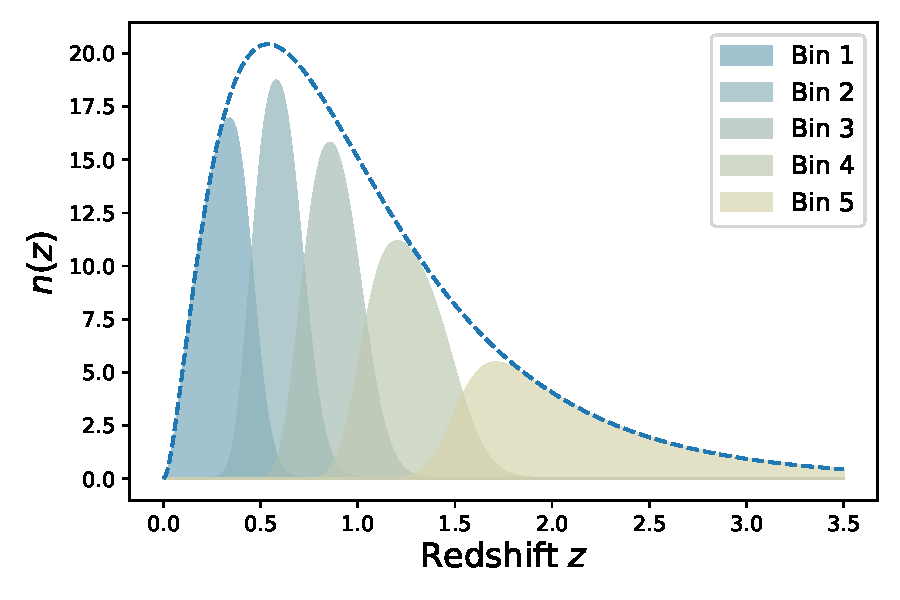
\includegraphics[width=\columnwidth]{figures/redshift_distribution_light.pdf}
    \caption{
     Source sample redshift distributions for each tomographic bin for LSST Y10. The number density on the y-axis is shown in arcmin$^2$.
    }
     \label{fig:redshift_distribution}
\end{figure}
%--------------------------------------------------------------------
%--------------------------------------------------------------------
%--------------------------------------------------------------------
%------------------------------------------------------------------
\section{Experiment}\label{Sec:experiment}
\subsection{Explicit Inference}
%--------------------------------------------------------------------
%--------------------------------------------------------------------
%--------------------------------------------------------------------
\subsubsection{Power spectrum}
Although this is not a full-field approach, we aim to compare the latest to a more standard approach. 
To obtain the probability distribution of the cosmological parameters using a summary-statistics-methods, we focus on the 2-point statistics, specifically, on the angular power spectra $C_{\ell}$.
The correlation between two generic tomographic bins $i$ and $j$ can be expressed as:
\begin{equation}
    \left \langle \kappa^{i}(\ell)\kappa^{j*}(\ell)\right \rangle =(2\pi)^2\delta_D(\ell-\ell')C_{\ell}^{ij},
\end{equation}
We assume a Gaussian likelihood with a cosmology-independent covariance matrix:
\begin{equation}
    \log{\mathcal{L}}(\bm{\theta})=-\frac{1}{2}[\bm{d}-\bm{\mu}(\bm{\theta})]^{T}\bm{C}^{-1}[\bm{d}-\bm{\mu}(\bm{\theta})].
\end{equation}
To compute the expected theoretical predictions $\bm{\mu}(\bm{\theta})$ we use the public library \href{https://github.com/DifferentiableUniverseInitiative/jax_cosmo}{\texttt{jax-cosmo}}. 
 The Covariance matrix $\bm{C}$ of the observables is computed at the fiducial cosmology, shown in \autoref{tab:prior}, using the same theoretical library. In {\texttt{jax-cosmo}}, the Gaussian covariance matrix is defined as:
\begin{equation}
    \text{Cov}(C_{\ell},C_{\ell}')=\frac{1}{f_{sky}(2 \ell+1)}\left(C_{\ell}+\frac{\sigma_{\epsilon}^2}{2n_s}\right)
\end{equation}
where $f_{sky}$ is the fraction of sky observed by the survey, and $n_s$ is the number density of galaxies. 
To obtain the data vector $\bm{d}$, containing the auto- and the cross-power spectra for each tomographic bin, we use the \href{https://lenstools.readthedocs.io/en/latest/lenstool} {\texttt{LensTools}} package \citep{2016A&C....17...73P} on a single noisy simulated map. 
%--------------------------------------------------------------------
%--------------------------------------------------------------------
%--------------------------------------------------------------------
\subsubsection{Full field and HMC}
The following steps outline our methods. We draw cosmological parameters from the priors illustrated in \autoref{tab:prior}. Given values for the cosmological parameters, we generate the log-normal field as described in the previous sections. So, in other words, the simulator becomes the physical model generating a non-linear representation of the convergence map. The measure of the convergence for each pixel and for each bin predicted from the physical model will differ from the ones from real observations due to the noise.  This is taken into account in the likelihood. Specifically, for LSST Y10 the number of galaxies for each pixel should be sufficiently high that for the central limit theorem, we can assume that the observation is characterized by a Gaussian noise $\sigma_n^2=\sigma_e^2/N_s$, with $N_s$ the total number of source galaxies per bin and pixel. Given $\sigma_n^2$ the variance of this Gaussian likelihood, its form in the log form can be expressed as:
\begin{equation}
    \log{\mathcal{L}}(\bm{\theta})=
    \sum_i^{N_{pix}} \sum_{j}^{N_{bins}} \log{P(\kappa^{obs}_{i,j}|\kappa_{i,j},\bm{\theta})}
    =\sum_i^{N_{pix}} \sum_{j}^{N_{bins}}\frac{[\kappa_{i,j}-\kappa^{obs}_{i,j}]^2}{2\sigma_n^2}
\end{equation}
Not relying on any summary statistics, the full-field approach typically results in a high-dimensional problem, requiring more sophisticated statistical techniques. To sample the posterior distribution for $\bm{\theta}$, we use a Hamiltonian Monte Carlo (HMC) algorithm. The HMC algorithm is particularly helpful in high-dimensional spaces where a large number of steps are required to effectively explore the space. It improves the sampling process by using the information contained in the gradients to guide the sampling process. Since the code is implemented in Jax, the gradients are accessible via automatic differentiation. 
%--------------------------------------------------------------------
%--------------------------------------------------------------------
%--------------------------------------------------------------------
\subsection{Implicit Inference}
%--------------------------------------------------------------------
%--------------------------------------------------------------------
%--------------------------------------------------------------------
\subsubsection{Need for data compression}
%--------------------------------------------------------------------
%--------------------------------------------------------------------
%--------------------------------------------------------------------
\subsubsection{Benchmark compression scheme}
There are several approaches available for training the compressor, and this section aims to provide an overview of these different methods used in previous works. 
In \autoref{Sec:results}, we will compare the outcomes of these various strategies. Specifically, using the same prior $p(\bm {\theta})$ for the cosmological parameter $\bm{\theta}$ and the simulator described in \autoref{Sec:results}, which samples $\bm {x}$ from $p(\bm{x}| \bm{\theta})$ and produces a set of mock observations $\bm{x_0}$, we will compare the posterior distribution $p(\bm{\theta}|\bm{x})$ obtained form each inference pipeline. This analysis will help to determine the optimal compression strategy, enabling us to extract the maximum amount of information possible given the fixed cosmological parameters.
%--------------------------------------------------------------------
\paragraph{\textcolor{violet}{Mean Square Error (MSE)}}
One of the most straightforward approaches adopted to train a Neural Network consists of minimizing the $L_2$ norm, or Mean Square Error (MSE). In this section, we demonstrate that this approach is equivalent to training the model to estimate the mean of the posterior distribution, namely:
\begin{equation}\label{Eq:mean_mse}
\left \langle \bm {\theta} \right \rangle_{p(\bm {\theta}|\bm{d})}=\operatorname*{argmin}_{\mathcal{F}(\bm{d})}\mathbb{E}_{p(\bm {\theta}|\bm {d})}[\left\Vert \bm {\theta}-\mathcal{F}(\bm{d})
 \right \Vert_{2}^{2}].
\end{equation}
To demonstrate \autoref{Eq:mean_mse}, we need to minimize the expected value of the $L_2$ norm with respect to $\mathcal{F}(\bm{d})$. Let us consider its derivative:
\begin{align}\label{Eq:moment_1}
   & \frac{\partial}{\partial \mathcal{F}(\bm{d}) }  \mathbb{E}_{p(\bm {\theta}|\bm{d}))}[(\bm {\theta}-\mathcal{F}(\bm{d}))^2] =  \\
    &
    \frac{\partial}{\partial \mathcal{F}(\bm{d}) }  \mathbb{E}_{p(\bm {\theta}|\bm {d})}[\bm {\theta}^2+\mathcal{F}(\bm{d})^2-2\bm {\theta}\mathcal{F}(\bm{d})] = \nonumber \\
    &
    \frac{\partial}{\partial \mathcal{F}(\bm{d}) }  [
    \mathbb{E}_{p(\bm {\theta}|\bm {d})}[\bm {\theta}^2]+\mathcal{F}(\bm{d})^2-2\mathcal{F}(\bm{d})\mathbb{E}_{p(\bm {\theta}|\bm {d})}[\bm {\theta}]]= \nonumber \\
    &2\mathcal{F}(\bm{d})-2 \mathbb{E}_{p(\bm {\theta}|\bm {d})}[\bm {\theta}]. \nonumber
\end{align}
Setting it equal to zero, we obtain the critical value:
\begin{equation}
    \mathcal{F}(\bm{d})= \mathbb{E}_{p(\bm {\theta}|\bm {d})}[\bm {\theta}]. 
\end{equation}
Considering the second-order derivative:
\begin{equation}\label{Eq:minimum_mean}
   \frac{\partial^2}{\partial^2 \mathcal{F}(\bm{d})}  \mathbb{E}_{p(\bm {\theta}|\bm {d})}[(\bm {\theta}-\mathcal{F}(\bm{d}))^2]=2, 
\end{equation}
we can assert that the critical value $\mathcal{F(\bm(\theta))}$ is also a minimum. 
Since 
\begin{equation}
    \mathbb{E}_{p(\bm {\theta}|\bm {d})}[\bm {\theta}|\bm{d}]= \left \langle \bm {\theta} \right \rangle_{p(\bm {\theta}|\bm{d})}
\end{equation}
it follows from \autoref{Eq:minimum_mean} the \autoref{Eq:mean_mse}.
%--------------------------------------------------------------------
\paragraph{\textcolor{violet}{Maximum Absolute Error (MAE)}}
Instead of minimizing the $L_2$ norm, these approaches focus on the $L_1$ norm or Mean Absolute Error (MAE). In this section, we demonstrate that this is equivalent to training the model to estimate the median of the posterior distribution.
By definition, the median of a probability density function $p(x)$ is a real number $m$ that satisfies:
\begin{equation}\label{Eq:definition_median}
\int_{\infty}^{m} p(x)dx=\int_{m}^{\infty}p(x)dx=\frac{1}{2}.
\end{equation}. 
The expectation value of the mean absolute error is defined as:
\begin{equation}
    \mathbb{E}[|x-m|]= \int_{\infty}^{\infty}p(x)|x-m|dx  
\end{equation}
which can be decomposed as
\begin{equation}
        \int_{\infty}^{m}p(x)|x-m|dx +\int_{m}^{\infty}p(x)|x-m|dx .
\end{equation}
To minimize this function with respect to $m$, we need to compute its derivative:
\begin{equation}\label{Eq:absolute_median}
    \frac{d\mathbb{E}[|x-m|]}{dm}=
    \frac{d}{dm}\int_{\infty}^{m}p(x)|x-m|dx +\frac{d}{dm}\int_{m}^{\infty}p(x)|x-m|dx. 
\end{equation}
Considering that $|x-m|=(x-m)$ for $m\le x$ and $|x-m|=(m-x)$ $m\ge x$, 
we can write \autoref{Eq:absolute_median} as:
\begin{equation}
    \frac{d\mathbb{E}[|x-m|]}{dm}=
    \frac{d}{dm}\int_{\infty}^{m}p(x)(m-x)dx +\frac{d}{dm}\int_{m}^{\infty}p(x)(x-m)dx .
\end{equation}
Using the Leibniz integral rule, we get:
\begin{align}
    &\frac{d\mathbb{E}[|x-m|]}{dm}= \\
    &
    p(x)(m-m)\frac{dm}{dm}+\int_{\infty}^{m}\frac{\partial}{\partial m}[p(x)(m-x)]dx + \nonumber \\
    & - p(x)(m-m)\frac{dm}{dm}+\int_{m}^{\infty}\frac{\partial}{\partial m}[p(x)(m-x)]dx \nonumber .
\end{align}
Setting the derivative to zero, we obtain:
\begin{equation}
    \frac{d\mathbb{E}[|x-m|]}{dm}= \int_{\infty}^{m} p(x)dx-\int_{m}^{\infty}p(x)dx =0.
\end{equation}
Thus,
\begin{equation}
\int_{\infty}^{m} p(x)dx=\int_{m}^{\infty}p(x)dx .
\end{equation}
Considering that
\begin{equation}
\int_{\infty}^{m} p(x)dx+\int_{m}^{\infty}p(x)dx=1,
\end{equation}
we obtain 
\begin{equation}\label{Eq:definition_median}
\int_{\infty}^{m} p(x)dx=\int_{m}^{\infty}p(x)dx=\frac{1}{2}.
\end{equation}
%--------------------------------------------------------------------
\paragraph{\textcolor{violet}{Gaussian Negative Log-Likelihood (GNLL)}}
%--------------------------------------------------------------------
\FL{I think we should have this section after the VMIM}

\FL{Recognizing that the uncertainty on different cosmological parameters will vary, a third
class of inverse variance weighted MSE was proposed in \cite{fluri2018cosmological} with the idea of
ensuring that each parameter contributes fairly to the overall loss by taking into account its uncertainty. The loss function typically takes the following form:
\begin{equation}
    \mathcal{L} = \frac{1}{2} \log(|\Sigma|) + \frac{1}{2}(t - \theta)^t \Sigma^{-1} (t - \theta) 
\end{equation}
where $t$ is the summary statistics and $\Sigma$ is the covariance matrix of representing the uncertainty on the cosmological parameters $\theta$. Both $t$ and $\Sigma$ can be outputs of the compression network, i.e. $f_\theta(x)=(t, \Sigma)$.

One recognizes here the expression of a Gaussian probability function, and this expression can thus be straightforwardly related to the VMIM case by simply assuming a Gaussian distribution as the variational approximation for the posterior $q(\theta | x) = \mathcal{N}(\theta; t, \Sigma)$.

This means that this loss function is actually sub-optimal for two reasons:
\begin{itemize}
    \item The summary extracted by the neural network $t$ is, similarly to the MSE case only an estimate of the mean of 
    the posterior distribution, which is not guaranteed to be sufficient.
    \item Because of the Gaussian variational assumption, the variational posterior can potentially be biased with respect to the true posterior, and thus the mean of this Gaussian approximation may be biased with respect to the true posterior mean.
\end{itemize}
 A simple MSE would thus seem to be preferable.
}
% A third possible scenario consists in minimizing the Negative Log Likelihood. First of all, let us stating that minimizing the negative log likelihood is equivalent to the Maximum Likelihood Estimation (MLE). The proof of this statement is straightforward. As suggested by the name, this optimization problem involves maximizing the likelihood distribution $p(\bm{x}|\bm{\theta})$
% \begin{equation}
%     \bm{\theta}_{ML}= \operatorname*{argmax}_{\bm{\theta}}p(\bm{x}|\bm{\theta}).
% \end{equation}
% where
% \begin{equation}
%     p(\bm{x}|\bm{\theta})= \prod_{i-1}^n p(x_i|\bm{\theta}).
% \end{equation}
% Applying the log function in this context is done for several reasons, e.g. reducing the potential of underflow when the likelihoods are small or allowing the conversion of a product into a summation. 
% Then, remembering that $-\log$ is strictly decreasing, the following are equivalent:
% \begin{equation}
%     \operatorname*{argmax}_{\bm{\theta}}\sum_{i-1}^n \log{p(x_i|\bm{\theta})}= \operatorname*{argmin}_{\bm{\theta}}-\sum_{i-1}^n \log{p(x_i|\bm{\theta})}.
% \end{equation}

%--------------------------------------------------------------------
\paragraph{\textcolor{violet}{Information Maximising Neural Networks (IMNNs)}}
%--------------------------------------------------------------------
\paragraph{\textcolor{violet}{Variational Mutual Information Maximization (VMIM)}}
The Variational Mutual Information Maximization (VMIM) has been used for cosmological inference problems for the first time by \citet{jeffrey2021likelihood}. This approach aims to maximize the mutual information $I(\bm{t}, \bm {\theta})$ between the cosmological parameters $\bm{\theta}$ and the summary statistics $\bm t$ by training a neural network with parameters $\phi$. 
Mathematically, it is defined as follows:
\begin{align}\label{Eq:mutual_information}
    I(\bm{t}, \bm {\theta}) &= D_{KL}(p(\bm {t}, \bm {\theta})||p(\bm {t})p(\bm {\theta})) \\ \nonumber
    &= \int d^n \bm{\theta} d^n \bm{t} p(\bm t, \bm \theta)\log{\left( \frac{ p(\bm {t}, \bm {\theta})}{ p(\bm {t}) p(\bm {\theta})} \right)} \\ \nonumber
    &= \int d^n \bm{\theta} d^n \bm{t} p(\bm t, \bm {\theta})\log{\left( \frac{ p(\bm {\theta} | \bm {t} )}{ p(\bm {\theta})} \right)} \\ \nonumber
        &= \int d^n \bm{\theta} d^n \bm{t} p(\bm t, \bm {\theta})\log{p(\bm {\theta} | \bm {t} )} - \int d^n \bm{\theta}  d^n \bm{t} p(\bm t, \bm {\theta})\log{p(\bm {\theta})} \\ \nonumber
    &= \int d^n \bm{\theta} d^n \bm{t} p(\bm t, \bm {\theta})\log{p(\bm {\theta} | \bm {t} )} - \int d^n \bm{\theta} p(\bm {\theta})\log{p(\bm {\theta})} \\ \nonumber
    &= \mathbb{E}_{p(\bm {t}, \bm {\theta})} [\log{p(\bm {\theta} | \bm {t} )}]- \mathbb{E}_{p(\bm {\theta})} [\log{p(\bm {\theta})}] \\ \nonumber
    &= \mathbb{E}_{p(\bm {t}, \bm {\theta})} [\log{p(\bm {\theta} | \bm {t} )}]- H(\bm {\theta});
\end{align}

where $D_{KL}$ is the Kullback-Leibler divergence \citep{kullback1951information}, $p(\bm {t}, \bm {\theta})$ is the joint probability distribution of summary statistics and cosmological parameters, and $H(\bm {\theta})$ represents the \textit{entropy} of the distribution of cosmological parameters.  
In other words, the mutual information measures the amount of information contained in the summary statistics $\bm t$ about the cosmological parameters $\bm \theta$.
Given the original high-dimensional data vector $\bm d$, the information $\bm t$ is extracted using $\bm {t}=F_{\bm {\phi}}(\bm {d})$. 
The goal is to find the parameters $\bm {\phi}$ that maximize the mutual information between the summary and cosmological parameters:
\begin{equation}
   \bm {\phi}^*= \operatorname*{argmax}_{\bm {\phi}} I(F_{\bm {\phi}}(\bm{d}), \bm {\theta}).
\end{equation}
However, the mutual information expressed in \autoref{Eq:mutual_information} is not tractable. To overcome this limitation,  several approaches have been developed, relying on tractable bounds that allow the training of a deep neural network to optimize the mutual information. In this work, we adopt the same strategy used by \citet{jeffrey2021likelihood} and use the variational lower bound \citep{barber2003information}:
\begin{equation}\label{Eq:variational_lower_bound}
    I(\bm{t}, \bm{\theta}) \ge \mathbb{E}_{p(\bm {t}, \bm {\theta})} [\log{q(\bm {\theta} |\bm{t} ; \bm{\phi}')}]- H(\bm {\theta}).
\end{equation}
Here, the variational conditional distribution $\log{q(\bm {\theta} |\bm{t} ; \bm{\phi}')}$ is introduced to approximate the true posterior distribution $p(\bm{\theta}|\bm {t})$. 
Since the entropy of the cosmological parameters is constant for a fixed training set, the optimization problem based on the lower bound in  \autoref{Eq:variational_lower_bound} can be written as:
\begin{equation}
    \operatorname*{argmax}_{\bm {\phi}, \bm {\phi}'}\mathbb{E}_{p(\bm {d}, \bm {\theta})} [\log{q(\bm {\theta} |F_{\bm {\phi}}(\bm {d}) ; \bm{\phi}')}].
\end{equation}
%--------------------------------------------------------------------
%--------------------------------------------------------------------
%--------------------------------------------------------------------
\subsubsection{Inference strategy}

To evaluate compression strategies, we propose a comparison of posteriors $p(\theta|s(x))$, where $s(x)$ is the summary statistic. Indeed, the more informative the summary statistics, the closer the posterior $p(\theta | s(x))$ is to the true posterior $p (\theta | x)$. To this end, we propose to do Neural Posterior Estimation (NPE) \justine{describe a bit more what it is, sbi method etc} that aims to directly learn from simulations the posterior distribution
\begin{equation}
    p(\theta | x) \propto \int p(x | \theta, z) p(z|\theta) p(\theta) dz\,.
\end{equation}
To achieve this, we train a  conditional Normalizing Flow (NF) \justine{as proposed by ... (REF) / neural simulation-based inference} $p_{\varphi} (\theta | s(x)) $ by minimizing the negative log-probability in $(\theta, s(x))$ space:
\begin{equation}
    \mathcal{L}_{\rm NLL} = \mathbb{E}_{p(\theta, s(x))} \left[ - \log p_{\varphi} (\theta | s(x))  \right].
    \label{eq:nll}
\end{equation}

\justine{talk about evaluation of approx posterior at a given obs}

By learning the posterior distribution for each statistic, we capture the significance of each statistic. This approach allows us to use the posterior distribution as a fair benchmark for comparison.
In particular, for each statistic we use the same NF architecture which is a RealNVP (REF) with 4 coupling layers, shift and scale parameters are learned using a neural network with 2 layers of 128 neurons, activation functions are $silu$ (REF).


\begin{center}
\begin{table*}
\begin{tabular}{ |p{3.5cm}|p{2cm}|p{3cm}|p{2.5cm}|p{4cm}|  }
 \hline
Reference & \makecell{Architecture\\ compressor}  & \makecell{Loss function} & \makecell{Inference \\ strategy} & \makecell{Output compressor}   \\
 \hline
            \citet{2018PhRvD..97j3515G} & \makecell{CNN} & \makecell{MAE} &  \makecell{Likelihood \\ analysis} &\makecell{$\sigma_8, \Omega_m$}  \\
 \hline
            \citet{fluri2018cosmological} & \makecell{CNN} & \makecell{MAE} & \makecell{Likelihood \\ analysis} &  \makecell{$\log{(\sigma_{\Omega_m}^2)},\log{(\sigma_{\sigma_8}^2)}$,
             \\
            $\tanh^{-1}{(\text{Corr}(\sigma_8,\Omega_m))}$,
             \\
            $\sigma_8,\Omega_m$} 
\\
\hline     
\rowcolor{lightgray}
            \citet{fluri2019cosmological} & \makecell{CNN} & \makecell{GNLL} & \makecell{Likelihood \\ analysis} & \makecell{$\sigma_8, \Omega_m, A_{IA}/10, L$  \\ with  $L:\Sigma^{-1}=LL^{T}$}
\\
\hline            
            \citet{ribli2018improved} & \makecell{CNN} & \makecell{MSE}  &\makecell{RMSE for \\ evaluation}  & \makecell{$\sigma_8, \Omega_m$}   
\\
\hline            
            \citet{ribli2019weak} & \makecell{CNN} & \makecell{MAE} & \makecell{Likelihood \\ analysis} & \makecell{$\sigma_8, \Omega_m$}   
\\            
\hline             
            \citet{PhysRevD.102.123506} & \makecell{CNN} & \makecell{MAE} & \makecell{Likelihood \\ analysis} & \makecell{$\sigma_8, \Omega_m$}   
\\
\hline 
\rowcolor{lightgray}
            \citet{jeffrey2021likelihood} & \makecell{\makecell{CNN} \\\makecell{CNN}+NF} & 
            \makecell{MSE \\ VMIM}
            & \makecell{PyDelfi} & \makecell{$\phi: F_{\phi}(\bm{d})=\bm{\theta}$ \\ with $\bm{\theta}=\Omega_m, \sigma_8$}    
\\            
\hline             
            \citet{fluri2021cosmological} & \makecell{GCNN} & \makecell{IMNN} & \makecell{GPABC} &  
\\
\hline      
\rowcolor{lightgray}

            \citet{fluri2022full} & \makecell{GCNN} & \makecell{IMNN} & \makecell{GPABC} &  
\\            
\hline 
            \citet{lu2022simultaneously} & \makecell{CNN} & \makecell{MSE} & \makecell{Likelihood \\ analysis}  & \makecell{$\Omega_m,S_8, A_{IA}/10,$ \\ rescaled \\ baryonic parameters \\ $(M_c,M_{1,0}, \eta, \beta)$}   
\\           
\hline 
            \citet{kacprzak2022deeplss} & \makecell{CNN} & \makecell{GNLL}  & \makecell{Likelihood \\ analysis}  & \makecell{WL: $\Sigma, \Omega_m, \sigma_8, A_{IA}, \eta_{IA}$ \\  GC:$\Sigma, \Omega_m, \sigma_8, b_g, r_g,\eta_{b_{g}}$ }
          
\\
\hline 
\rowcolor{lightgray}
            \citet{lu2023cosmological} & \makecell{CNN} & \makecell{MSE} & \makecell{Likelihood \\ analysis}  & \makecell{$\Omega_m,S_8,A_{IA}/10,$\\ rescaled baryonic \\ parameters: $M_c,M_{1,0}, \eta, \beta$} 
\end{tabular}
\label{tab:biblio_survey}
\end{table*}
\end{center}



%--------------------------------------------------------------------
\section{Results}\label{Sec:results}
\begin{figure*}
    \centering
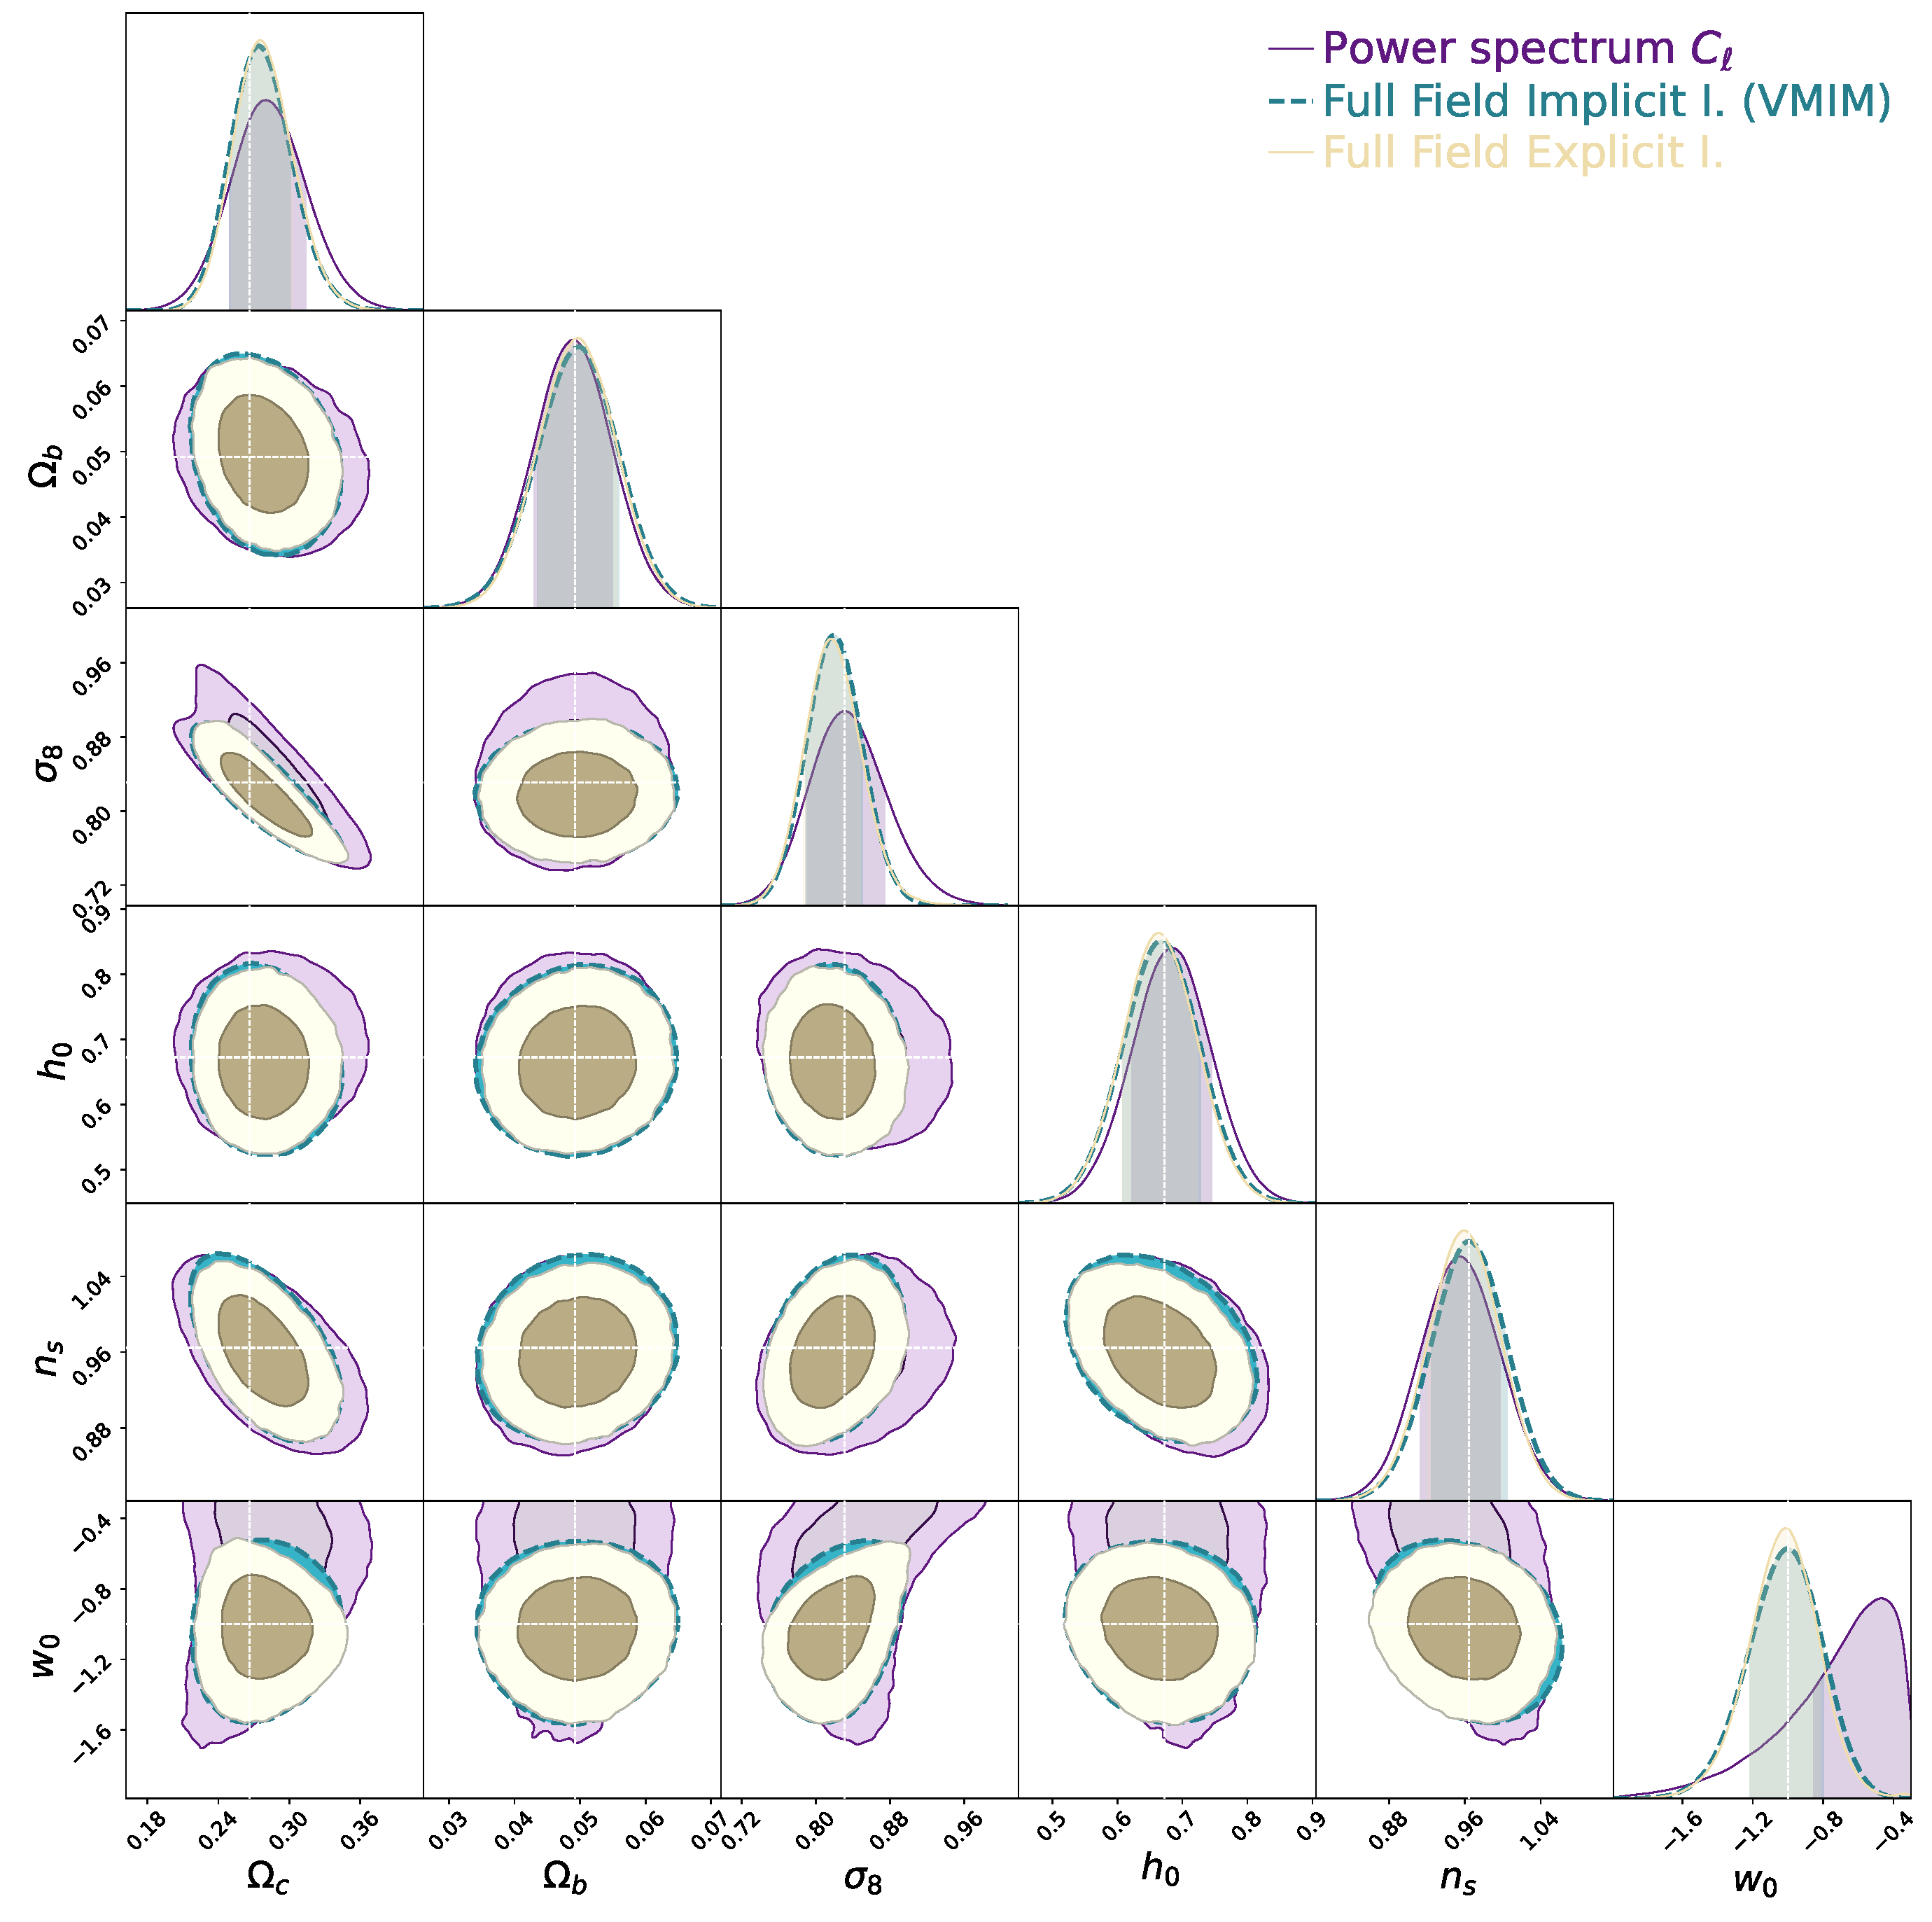
\includegraphics[width=\textwidth]{figures/contours_posterior_imp_ex_ps.pdf}
    \caption{
Constraints on the $\Lambda$CDM parameter space as found in the LSST Y10 survey setup. The constraints are obtained by applying the $C_{\ell}$ (light blue contours), the full field explicit inference (yellow contours), and the full field implicit inference strategy (violet contours), described in \autoref{Sec:experiment}.
The contours show the $68\%$ and the $95\%$  confidence regions. The dashed white lines define the true parameter values.}
\label{fig:contours_posterior_imp_ex_ps}
\end{figure*}
%--------------------------------------------------------------------
\section{Conclusions}
%--------------------------------------------------------------------
%--------------------------------------------------------------------
\begin{acknowledgements}
This work was granted access to the HPC/AI resources of IDRIS under the allocation 2022-AD011013922 made by GENCI.
\end{acknowledgements}

\bibliographystyle{aa} % style aa.bst
\bibliography{paper/biblio} 
\end{document}